\documentclass{article}

\usepackage{fancyhdr}
\usepackage{extramarks}
\usepackage{amsmath}
\usepackage{amsthm}
\usepackage{amsfonts}
\usepackage{tikz}
\usepackage[plain]{algorithm}
\usepackage{algpseudocode}
\usepackage{listings}
\usepackage{minted}
\usepackage[utf8]{inputenc}
\usepackage[english]{babel}
\usetikzlibrary{automata,positioning}
\usepackage{graphicx}
\usepackage{amsmath}
\usepackage{tikz}
\usetikzlibrary{positioning}
%
% Basic Document Settings
%


\topmargin=-0.45in
\evensidemargin=0in
\oddsidemargin=0in
\textwidth=6.5in
\textheight=9.0in
\headsep=0.25in

\linespread{1.1}

\pagestyle{fancy}
\lhead{\hmwkClass\ (\hmwkClassInstructor): \hmwkTitle}
\chead{\hspace{4.8in}\hmwkAuthorName}
\rhead{\firstxmark}
\lfoot{\lastxmark}
\cfoot{\thepage}

\renewcommand\headrulewidth{0.4pt}
\renewcommand\footrulewidth{0.4pt}

\setlength\parindent{0pt}

%
% Create Problem Sections
%

\newcommand{\enterProblemHeader}[1]{
    \nobreak\extramarks{}{Problem \arabic{#1} continued on next page\ldots}\nobreak{}
    \nobreak\extramarks{Problem \arabic{#1} (continued)}{Problem \arabic{#1} continued on next page\ldots}\nobreak{}
}

\newcommand{\exitProblemHeader}[1]{
    \nobreak\extramarks{Problem \arabic{#1} (continued)}{Problem \arabic{#1} continued on next page\ldots}\nobreak{}
    \stepcounter{#1}
    \nobreak\extramarks{Problem \arabic{#1}}{}\nobreak{}
}

\setcounter{secnumdepth}{0}
\newcounter{partCounter}


%
% Homework Problem Environment
%
% This environment takes an optional argument. When given, it will adjust the
% problem counter. This is useful for when the problems given for your
% assignment aren't sequential. See the last 3 problems of this template for an
% example.
%


%
% Homework Details
%   - Title
%   - Due date
%   - Class
%   - Section/Time
%   - Instructor
%   - Author
%

\newcommand{\hmwkTitle}{Homework 5}
\newcommand{\hmwkDueDate}{Monday, April 4, 2016}
\newcommand{\hmwkClass}{DS-GA 1003}
\newcommand{\hmwkClassInstructor}{Professor David Ronsenberg}
\newcommand{\hmwkAuthorName}{Yuhao Zhao}
\newcommand{\hmwknetid}{Yz3085}
\newcommand{\hmwksubtitle}{Trees and Boosting}
\newcommand{\gihub}{See complete code at: \textit{git@github.com:cryanzpj/1003.git}}
%
% Title Page
%

\title{
    \vspace{2in}
    \textmd{\textbf{\hmwkClass:\ \hmwkTitle \\ \hmwksubtitle }}\\
    \vspace{1in}
    \normalsize\vspace{0.1in}\small{Due\ on\ \hmwkDueDate}\\
    \vspace{0.1in}\large{\textit{\hmwkClassInstructor}}\\
    \vspace{3in}
    \author{\textbf{\hmwkAuthorName} \\ \textbf{\hmwknetid }\\ }
    \vspace{0.2in}
    \gihub
}



\date{}

\renewcommand{\part}[1]{\textbf{\large Part \Alph{partCounter}}\stepcounter{partCounter}\\}

%
% Various Helper Commands
%

% Useful for algorithms
\newcommand{\alg}[1]{\textsc{\bfseries \footnotesize #1}}

% For derivatives
\newcommand{\deriv}[1]{\frac{\mathrm{d}}{\mathrm{d}x} (#1)}

% For partial derivatives
\newcommand{\pderiv}[2]{\frac{\partial}{\partial #1} (#2)}

% Integral dx
\newcommand{\dx}{\mathrm{d}x}

% Alias for the Solution section header
\newcommand{\solution}{\textbf{\large Solution}}

% Probability commands: Expectation, Variance, Covariance, Bias
\newcommand{\E}{\mathrm{E}}
\newcommand{\Var}{\mathrm{Var}}
\newcommand{\Cov}{\mathrm{Cov}}
\newcommand{\Bias}{\mathrm{Bias}}





\newenvironment{problem}[2][$\bullet$]{\begin{trivlist}\large
		\item[\hskip \labelsep {\bfseries #1}\hskip \labelsep {\bfseries #2.}]}  {\end{trivlist}}

\newenvironment{sub}[2][$-$]{\begin{trivlist}
		\item[\hskip \labelsep {\bfseries #1}\hskip \labelsep {\bfseries #2.}]}  {\end{trivlist}}
\newenvironment{lemma}[2][Lemma]{\begin{trivlist}
		\item[\hskip \labelsep {\bfseries #1}\hskip \labelsep {\bfseries #2.}]}{\end{trivlist}}
\newenvironment{exercise}[2][Exercise]{\begin{trivlist}
		\item[\hskip \labelsep {\bfseries #1}\hskip \labelsep {\bfseries #2.}]}{\end{trivlist}}

\newenvironment{question}[2][Question]{\begin{trivlist}
		\item[\hskip \labelsep {\bfseries #1}\hskip \labelsep {\bfseries #2.}]}{\end{trivlist}}
\newenvironment{corollary}[2][Corollary]{\begin{trivlist}
		\item[\hskip \labelsep {\bfseries #1}\hskip \labelsep {\bfseries #2.}]}{\end{trivlist}}

\begin{document}

\maketitle

\pagebreak
\section{2 Decision Trees}
\begin{problem}{2.1 Trees on the Banana Dataset}
\end{problem}

\begin{sub}{2.1.1}
\end{sub}

\begin{minted}{python}
import numpy as np
import scipy as sp
import matplotlib.pyplot as plt
from sklearn.tree import DecisionTreeClassifier

file_train = open('data/banana_train.csv')
file_test = open('data/banana_test.csv')

train = np.array(map(lambda x: x[:2] + [x[-1].strip()],
			 [i.split(',') for i in file_train]), dtype='float')
test = np.array(map(lambda x: x[:2] + [x[-1].strip()],
			 [i.split(',') for i in file_test]), dtype='float')

y_train = np.array([0 if i == -1 else 1 for i in train[:, 0]])
y_test = np.array([0 if i == -1 else 1 for i in test[:, 0]])
X_train = train[:, 1:]
X_test = test[:, 1:]
\end{minted}

\begin{sub}{2.1.2}
\end{sub}

\begin{minted}{python}
n_classes = 2
plot_colors = "bry"
plot_step = 0.02

error = np.zeros((2, 10))

for i in xrange(1, 11):
	idx = np.arange(X_train.shape[0])
	np.random.seed(1)
	np.random.shuffle(idx)
	X = X_train[idx]
	y = y_train[idx]

	mean = X.mean(axis=0)
	std = X.std(axis=0)
	X = (X - mean) / std
	
	clf = DecisionTreeClassifier(max_depth=i).fit(X, y)
	plt.subplot(2, 5, i)
	x_min, x_max = X[:, 0].min() - 1, X[:, 0].max() + 1
	y_min, y_max = X[:, 1].min() - 1, X[:, 1].max() + 1
	xx, yy = np.meshgrid(np.arange(x_min, x_max, plot_step),
	np.arange(y_min, y_max, plot_step))
	
	Z = clf.predict(np.c_[xx.ravel(), yy.ravel()])
	Z = Z.reshape(xx.shape)
	
	training_error = np.sum(np.equal(clf.predict(X_train), 
					1 - y_train)) / float(y_train.shape[0])
	testing_error = np.sum(np.equal(clf.predict(X_test), 
						1 - y_test)) / float(y_test.shape[0])
	error[:, i - 1] = np.array([training_error, testing_error])
	
	cs = plt.contourf(xx, yy, Z, cmap=plt.cm.Paired)
	
	plt.axis("tight")
	
	for i, color in zip(range(n_classes), plot_colors):
		idx = np.where(y == i)
		plt.scatter(X[idx, 0], X[idx, 1], c=color, label=str(i),
				cmap=plt.cm.Paired)
	
	plt.axis("tight")
	plt.legend(fontsize=10)
plt.suptitle('Decision surface for different depth')
plt.show()
\end{minted}

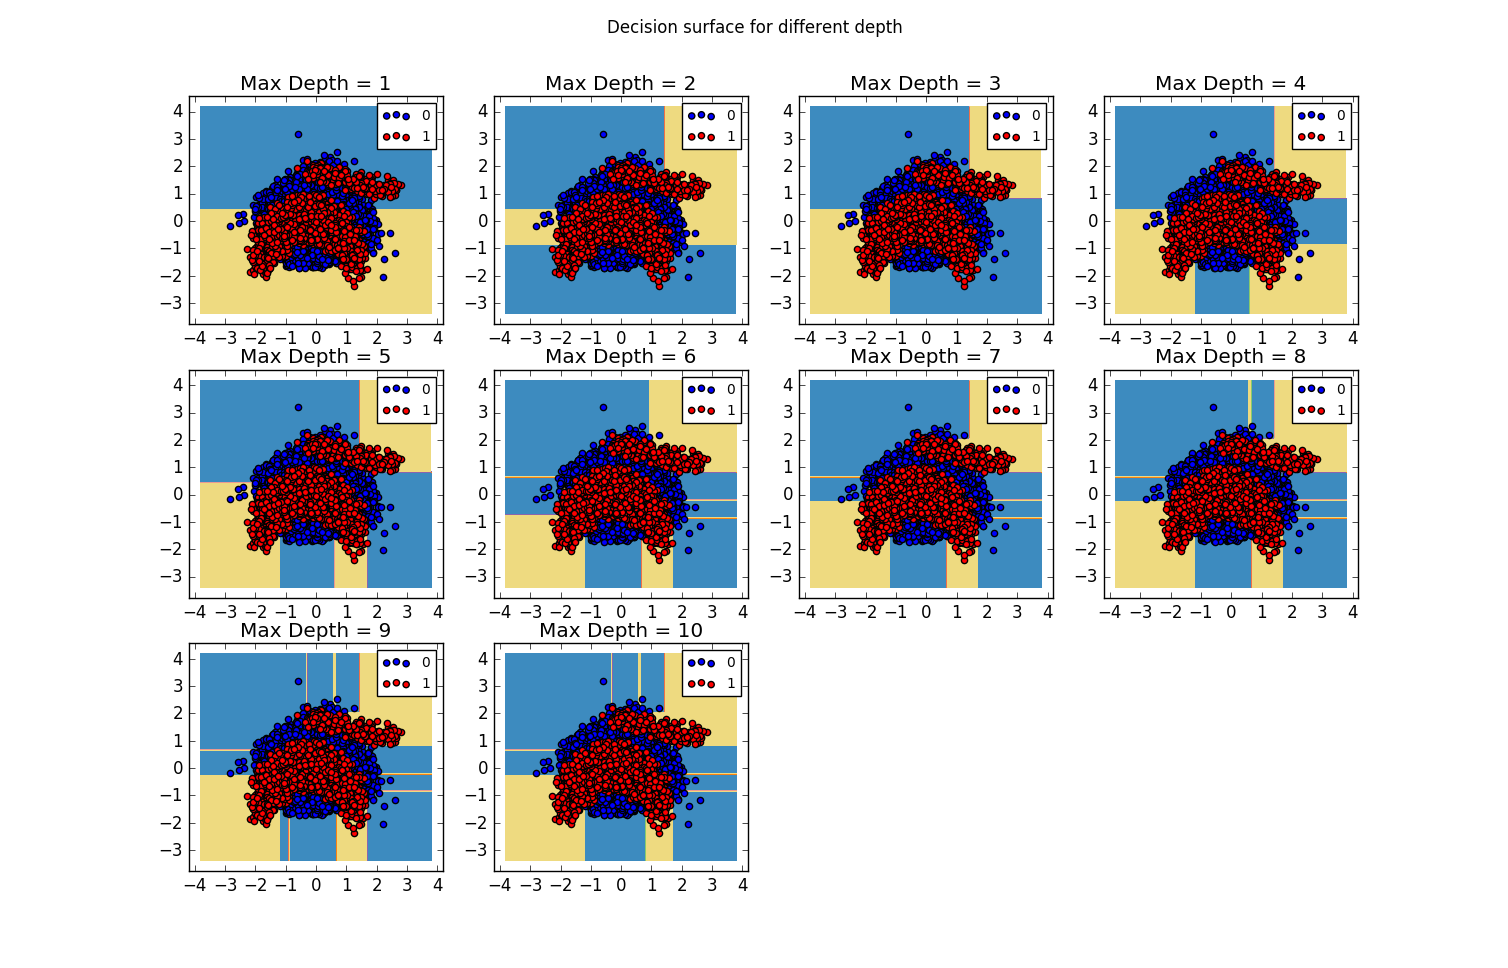
\includegraphics[width = 7.5in]{2_1_2.png}




\end{document}
